\usetikzlibrary{arrows.meta,positioning,matrix,calc,patterns}
\begin{frame}<1>[fragile,label=caseEvol]{case study: Evol}
    \begin{itemize}
    \item via Lakhatia et al, ``Are metamorphic viruses really invincible?'', Virus Bulletin, Jan 2005.
    \item ``\myemph{mutation engine}''
        \begin{itemize}
        \item run as part of propagating the virus
        \end{itemize}
    \end{itemize}
    \begin{tikzpicture}
        \tikzset{
            every node/.style={font=\small,align=center},
            hiOn/.style={alt=<#1>{red,ultra thick}{}},
            ignore/.style={alt=<4>{}{}}
        }
        \path node[draw,hiOn=2] (disasm) {disassemble} -- ++(2.5cm,0) node (lens) {instr. \\ lengths} -- ++(2cm,0) node[draw,hiOn=3] (xform) {transform}
              -- ++(2cm,0) node[draw,hiOn=4] (reloc) {relocate};
        \node (origCode) at ([xshift=-2cm,yshift=1cm]disasm.north) {code};
        \node (finalCode) at ([xshift=2cm,yshift=-1cm]reloc.south) {code};
        \begin{scope}[thick,-Latex]
        \draw (origCode) |- (disasm);
        \draw (disasm) -- (lens);
        \draw (lens) -- (xform);
        \draw (xform) -- (reloc);
        \draw (reloc) -| (finalCode);
        \end{scope}
    \end{tikzpicture}
\end{frame}

\againframe<2>{caseEvol}

\begin{frame}{Evol instruction lengths}
    \begin{itemize}
    \item sounds really complicated?
    \item virus only handles instructions it has:
        \begin{itemize}
        \item about 61 opcodes, 32 of them identified by first four bits
            \begin{itemize}
            \item e.g. opcode {\tt 0x7\textit{x}} -- conditional jump
            \end{itemize}
        \end{itemize}
    \item no prefixes, no floating point
    \item only {\tt \%reg} or {\tt \$constant} or {\tt offset(\%reg)}
    \end{itemize}
\end{frame}

\againframe<3>{caseEvol}

\newsavebox{\evolXExStart}
\begin{lrbox}{\evolXExStart}
\lstset{language=myasm,style=small}
\begin{lstlisting}
mov %eax, 8(%ebp)
\end{lstlisting}
\end{lrbox}

\newsavebox{\evolXExExpand}
\begin{lrbox}{\evolXExExpand}
\lstset{language=myasm,style=small}
\begin{lstlisting}
push %ecx
mov %ebp, %ecx
add $0x12, %ecx
mov %eax, -0xa(%ecx)
pop %ecx
\end{lstlisting}
\end{lrbox}

\begin{frame}[fragile,label=evolXform]{Evol transformations}
    \begin{itemize}
    \item some stuff left alone
    \item static or random one of $N$ transformations
    \item example:
    \end{itemize}
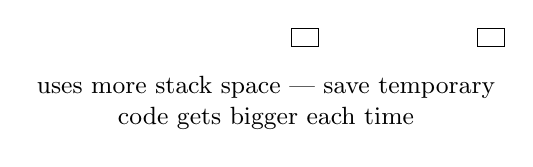
\begin{tikzpicture}
\tikzset{
    every node/.style={font=\small,align=center}
}
\node[draw] (movebpEight) {
\usebox{\evolXExStart}
};

\node[draw,right=2cm of movebpEight] (movebpExpand) {
\usebox{\evolXExExpand}
};
\node[anchor=north east] at ([yshift=-.25cm]movebpExpand.south east) {
    uses more stack space --- save temporary \\
    code gets bigger each time
};
\end{tikzpicture}
\imagecredit{Lakhotia et al., ``Are metamorphic viruses really invincible?'', Virus Bulletin, Jan 2005}
\end{frame}

\againframe<4>{caseEvol}

